\documentclass[12pt,a4paper]{article}

% ---------------------------------------------
%  PACKAGES
% ---------------------------------------------
\usepackage[utf8]{inputenc}
\usepackage[T1]{fontenc}
\usepackage[margin=2.5cm]{geometry}
\usepackage{xcolor}
\usepackage{listings}
\usepackage{tikz}
\usetikzlibrary{automata, positioning, arrows.meta, shapes.geometric}
\usepackage{tcolorbox}
\tcbuselibrary{skins, breakable, listingsutf8}
\usepackage{hyperref}
\usepackage{amsmath}
\usepackage{booktabs}
\usepackage{array}
\usepackage{enumitem}
\usepackage{pifont}
% -- Icon aliases (replacing fontawesome5 with pifont dingbats) ----------
\newcommand{\faLock}{\ding{108}}
\newcommand{\faUnlock}{\ding{109}}
\newcommand{\faStar}{\ding{72}}
\newcommand{\faCheck}{\ding{51}}
\newcommand{\faCheckCircle}{\ding{51}}
\newcommand{\faTimesCircle}{\ding{55}}
\newcommand{\faCheckSquare}{\ding{52}}
\newcommand{\faExclamationTriangle}{\ding{115}}
\usepackage{titlesec}
\usepackage{fancyhdr}
\usepackage{mdframed}
\usepackage{multirow}

% ---------------------------------------------
%  COLOURS
% ---------------------------------------------
\definecolor{vhdlbg}     {RGB}{18,  26,  38}
\definecolor{vhdlkw}     {RGB}{86,  156, 214}   % keywords
\definecolor{vhdlstring} {RGB}{206, 145, 120}   % strings / literals
\definecolor{vhdlcomment}{RGB}{106, 153, 85}    % comments
\definecolor{vhdltype}   {RGB}{78,  201, 176}   % types
\definecolor{vhdlnum}    {RGB}{181, 206, 168}   % numbers
\definecolor{vhdltext}   {RGB}{212, 212, 212}   % normal text

\definecolor{accentblue} {RGB}{0,   120, 215}
\definecolor{accentgreen}{RGB}{16,  163, 127}
\definecolor{accentred}  {RGB}{220, 53,  69}
\definecolor{accentyellow}{RGB}{255,193, 7}
\definecolor{sectionbg}  {RGB}{240, 248, 255}
\definecolor{notebg}     {RGB}{255, 249, 230}
\definecolor{errorbg}    {RGB}{255, 235, 238}
\definecolor{successbg}  {RGB}{232, 255, 232}

% ---------------------------------------------
%  VHDL LISTING STYLE
% ---------------------------------------------
\lstdefinelanguage{VHDL2}{
  morekeywords=[1]{
    library, use, entity, is, port, in, out, inout, buffer,
    architecture, of, begin, end, signal, type, subtype,
    process, variable, constant, generic, map, wait,
    if, then, elsif, else, case, when, others,
    and, or, not, nor, nand, xor, xnor,
    rising\_edge, falling\_edge,
    std\_logic, std\_logic\_vector, bit, boolean, integer,
    natural, positive, unsigned, signed,
    all, null, downto, to, range
  },
  morekeywords=[2]{
    std\_logic\_1164, ieee, numeric\_std, std\_logic\_arith,
    std\_logic\_unsigned
  },
  sensitive=false,
  morecomment=[l]{--},
  morestring=[b]",
}

\lstdefinestyle{vhdlstyle}{
  language         = VHDL2,
  backgroundcolor  = \color{vhdlbg},
  basicstyle       = \ttfamily\small\color{vhdltext},
  keywordstyle     = [1]{\color{vhdlkw}\bfseries},
  keywordstyle     = [2]{\color{vhdltype}},
  commentstyle     = \color{vhdlcomment}\itshape,
  stringstyle      = \color{vhdlstring},
  numberstyle      = \tiny\color{vhdlnum},
  numbers          = left,
  numbersep        = 10pt,
  stepnumber       = 1,
  tabsize          = 4,
  showstringspaces = false,
  breaklines       = true,
  frame            = none,
  xleftmargin      = 15pt,
  xrightmargin     = 5pt,
  aboveskip        = 0pt,
  belowskip        = 0pt,
}

% ---------------------------------------------
%  TCOLORBOX STYLES
% ---------------------------------------------
\tcbset{
  vhdlbox/.style={
    enhanced, breakable,
    colback   = vhdlbg,
    colframe  = accentblue!60!black,
    fonttitle = \bfseries\sffamily\color{white},
    coltitle  = white,
    attach boxed title to top left={yshift=-2mm, xshift=4mm},
    boxed title style={colback=accentblue!80!black, rounded corners},
    arc       = 4pt,
    top       = 6pt,
    bottom    = 6pt,
  },
  notebox/.style={
    enhanced, breakable,
    colback  = notebg,
    colframe = accentyellow!80!black,
    fonttitle= \bfseries\sffamily,
    arc      = 3pt,
  },
  errorbox/.style={
    enhanced, breakable,
    colback  = errorbg,
    colframe = accentred,
    fonttitle= \bfseries\sffamily\color{accentred},
    arc      = 3pt,
  },
  successbox/.style={
    enhanced, breakable,
    colback  = successbg,
    colframe = accentgreen,
    fonttitle= \bfseries\sffamily\color{accentgreen},
    arc      = 3pt,
  },
}

% ---------------------------------------------
%  TITLE FORMATTING
% ---------------------------------------------
\titleformat{\section}
  {\Large\bfseries\sffamily\color{accentblue}}
  {\thesection}{1em}{}
  [\color{accentblue}\titlerule]

\titleformat{\subsection}
  {\large\bfseries\sffamily\color{accentblue!80!black}}
  {\thesubsection}{1em}{}

\titleformat{\subsubsection}
  {\normalsize\bfseries\sffamily\color{accentblue!60!black}}
  {\thesubsubsection}{1em}{}

% ---------------------------------------------
%  HEADER / FOOTER
% ---------------------------------------------
\pagestyle{fancy}
\fancyhf{}
\fancyhead[L]{\sffamily\small\color{gray} FSM in VHDL --- Complete Guide}
\fancyhead[R]{\sffamily\small\color{gray} DSD Lab}
\fancyfoot[C]{\sffamily\small\thepage}
\renewcommand{\headrulewidth}{0.4pt}

% ---------------------------------------------
%  TIKZ FSM STYLE
% ---------------------------------------------
\tikzset{
  fsmstate/.style={
    circle, draw=accentblue, very thick,
    minimum size=1.1cm, font=\sffamily\bfseries,
    fill=accentblue!10
  },
  fsminitial/.style={
    circle, draw=accentgreen, very thick,
    minimum size=1.1cm, font=\sffamily\bfseries,
    fill=accentgreen!15
  },
  fsmfinal/.style={
    circle, draw=accentred, very thick,
    double, double distance=2pt,
    minimum size=1.1cm, font=\sffamily\bfseries,
    fill=accentred!10
  },
  fsmarrow/.style={
    ->, >=Stealth, thick, color=gray!80!black
  },
  fsmlabel/.style={
    font=\sffamily\small, fill=white, inner sep=1pt
  },
}

% ---------------------------------------------
%  HELPER COMMANDS
% ---------------------------------------------
\newcommand{\vhdlkeyword}[1]{\textcolor{vhdlkw}{\texttt{\textbf{#1}}}}
\newcommand{\levelbadge}[2]{%
  \begin{tcolorbox}[colback=#2!15, colframe=#2, arc=20pt,
    left=4pt, right=4pt, top=2pt, bottom=2pt,
    width=\linewidth, boxrule=1pt]
    \centering\sffamily\bfseries\large #1
  \end{tcolorbox}%
}

% ---------------------------------------------
%  DOCUMENT START
% ---------------------------------------------
\begin{document}

% ==============================================
%  TITLE PAGE
% ==============================================
\begin{titlepage}
  \centering
  \vspace*{2cm}

  {\Huge\bfseries\sffamily\color{accentblue}
    Finite State Machines\\\medskip
    \large in VHDL}

  \vspace{0.5cm}
  \noindent\rule{0.8\linewidth}{1.5pt}
  \vspace{0.5cm}

  {\large\sffamily A Complete Hands-On Guide\\
  \textit{From Beginner to Advanced}}

  \vspace{1.5cm}

  \begin{tcolorbox}[colback=vhdlbg, colframe=accentblue!60!black,
      arc=8pt, width=0.85\linewidth]
    \lstset{style=vhdlstyle, numbers=none}
    \begin{lstlisting}
-- The skeleton you will master in this guide
architecture myfsm of fsm is
    type state_type is (S0, S1, S2, S3);
    signal state, nextState : state_type;
begin
    -- Process 1 : State Register
    process (reset, clk) ...

    -- Process 2 : Next-State  +  Output Logic
    process (state, X) ...
end myfsm;
    \end{lstlisting}
  \end{tcolorbox}

  \vspace{1.5cm}

  \begin{tabular}{ll}
    \toprule
    \textbf{Subject}  & Digital System Design (DSD) \\
    \textbf{Tool}     & Intel Quartus Prime / ModelSim \\
    \textbf{VHDL Std} & IEEE 1164 \\
    \textbf{Levels}   & 1 (Beginner) $\rightarrow$ 6 (Advanced) \\
    \bottomrule
  \end{tabular}

  \vfill
  {\small\color{gray} This guide follows the 2-process Mealy/Moore template
   and the exact coding style used in your lab sessions.}
\end{titlepage}

\tableofcontents
\newpage

% ==============================================
%  SECTION 1  —  THEORY FUNDAMENTALS
% ==============================================
\section{FSM Theory --- The Foundation}

\subsection{What is a Finite State Machine?}

A \textbf{Finite State Machine (FSM)} is a sequential circuit that:
\begin{itemize}[leftmargin=1.5cm]
  \item Has a \textbf{finite} number of states.
  \item Is always in \textbf{exactly one} state at any clock edge.
  \item Moves to a \textbf{next state} based on the current state and inputs.
  \item Produces \textbf{outputs} based on the state (and sometimes inputs).
\end{itemize}

\begin{tcolorbox}[notebox, title={Core Formula}]
  \[
    \text{Next State} = f(\text{Current State},\ \text{Inputs})
  \]
  \[
    \text{Output} = g(\text{Current State})
    \quad \text{[Moore]} \quad \text{or} \quad
    g(\text{Current State},\ \text{Inputs}) \quad \text{[Mealy]}
  \]
\end{tcolorbox}

\subsection{Moore vs Mealy --- Key Difference}

\begin{center}
\begin{tabular}{>{\bfseries}l  p{5.5cm}  p{5.5cm}}
  \toprule
  & \textbf{Moore Machine} & \textbf{Mealy Machine} \\
  \midrule
  Output depends on & State only & State \textbf{and} Inputs \\
  Output changes    & Only at clock edge & Can change with input (async) \\
  States needed     & Usually more & Usually fewer \\
  Diagram label     & State bubble holds output & Arrow/transition holds output \\
  VHDL output       & Assigned in state register process or separate & Assigned inside combinational process \\
  \bottomrule
\end{tabular}
\end{center}

\subsection{The 2-Process Template (Your Style)}

Every FSM you write in this guide uses \textbf{exactly two processes}:

\begin{center}
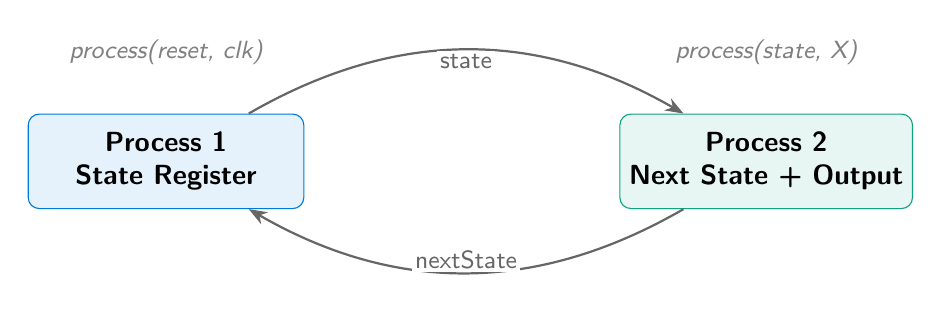
\begin{tikzpicture}[node distance=2cm]
  \node[draw=accentblue, fill=accentblue!10, rounded corners,
        minimum width=3.5cm, minimum height=1.2cm, align=center,
        font=\sffamily\bfseries] (sr)
        {Process 1\\State Register};
  \node[draw=accentgreen, fill=accentgreen!10, rounded corners,
        minimum width=3.5cm, minimum height=1.2cm, align=center,
        font=\sffamily\bfseries, right=4cm of sr] (ns)
        {Process 2\\Next State + Output};
  \draw[fsmarrow, bend left=30] (ns) to node[fsmlabel, above]{nextState} (sr);
  \draw[fsmarrow, bend left=30] (sr) to node[fsmlabel, below]{state} (ns);
  \node[above=0.5cm of sr, font=\sffamily\small\itshape, color=gray]
        {process(reset, clk)};
  \node[above=0.5cm of ns, font=\sffamily\small\itshape, color=gray]
        {process(state, X)};
\end{tikzpicture}
\end{center}

\begin{itemize}
  \item \textbf{Process 1} --- clocked, sensitive to \texttt{reset} and \texttt{clk}.
        Contains the flip-flops. Simple; never changes.
  \item \textbf{Process 2} --- combinational, sensitive to \texttt{state} and all \textbf{inputs}.
        Contains the \textit{brain} of your FSM.
\end{itemize}

\newpage

% ==============================================
%  SECTION 2  —  LEVEL 1
% ==============================================
\section{Level 1 --- Your First FSM (Toggle Machine)}

\levelbadge{\faLock\ Level 1 $\cdot$ Beginner --- 2 States, 1 Input, 1 Output}{accentgreen}

\subsection{Problem}

Design a \textbf{Moore FSM} that toggles output \texttt{Z} every time input \texttt{X = 1}.
The machine resets to state \texttt{S0} (\texttt{Z = 0}) when \texttt{reset = 1}.

\subsection{State Diagram}

\begin{center}
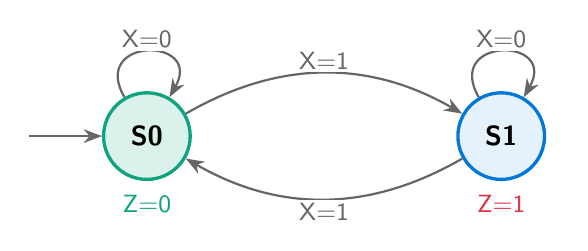
\begin{tikzpicture}[node distance=4.5cm]
  % States
  \node[fsminitial] (S0) {S0};
  \node[fsmstate, right of=S0] (S1) {S1};

  % Moore outputs inside states
  \node[below=0.05cm of S0, font=\sffamily\small\color{accentgreen}]{Z=0};
  \node[below=0.05cm of S1, font=\sffamily\small\color{accentred}]{Z=1};

  % Reset arrow
  \draw[fsmarrow] (-1.5,0) -- (S0);

  % Transitions
  \draw[fsmarrow, bend left=30] (S0) to node[fsmlabel, above]{X=1} (S1);
  \draw[fsmarrow, bend left=30] (S1) to node[fsmlabel, below]{X=1} (S0);
  \draw[fsmarrow] (S0) to[out=120, in=60, looseness=4]
        node[fsmlabel, above]{X=0} (S0);
  \draw[fsmarrow] (S1) to[out=120, in=60, looseness=4]
        node[fsmlabel, above]{X=0} (S1);
\end{tikzpicture}
\end{center}

\begin{tcolorbox}[notebox, title={Reading State Diagrams}]
  \begin{itemize}
    \item \textcolor{accentgreen}{\textbf{Green circle}} = Initial state (loaded on reset).
    \item \textbf{Arrow label} = input condition to take that transition.
    \item \textbf{Text inside bubble} = Moore output for that state.
    \item \textbf{Self-loop} = stay in same state when condition is met.
  \end{itemize}
\end{tcolorbox}

\subsection{State Table}

\begin{center}
\begin{tabular}{cccc}
  \toprule
  \textbf{Current State} & \textbf{Input X} & \textbf{Next State} & \textbf{Output Z} \\
  \midrule
  S0 & 0 & S0 & 0 \\
  S0 & 1 & S1 & 0 \\
  S1 & 0 & S1 & 1 \\
  S1 & 1 & S0 & 1 \\
  \bottomrule
\end{tabular}
\end{center}

\subsection{VHDL Implementation}

\begin{tcolorbox}[vhdlbox, title={Level 1 --- toggle\_fsm.vhd}]
\begin{lstlisting}[style=vhdlstyle]
library ieee;
use ieee.std_logic_1164.all;

entity toggle_fsm is
    port (
        clk   : in  std_logic;   -- clock
        reset : in  std_logic;   -- async active-high reset
        X     : in  std_logic;   -- input
        Z     : out std_logic    -- output
    );
end toggle_fsm;

architecture myfsm of toggle_fsm is
    -- state encoding
    type state_type is (S0, S1);

    -- signals
    signal state, nextState : state_type;

begin

    -- -----------------------------------------
    -- Process 1 : State Register (clocked)
    -- -----------------------------------------
    process (reset, clk)
    begin
        if reset = '1' then
            state <= S0;              -- async reset to initial state
        elsif rising_edge(clk) then
            state <= nextState;       -- advance on clock edge
        end if;
    end process;

    -- -----------------------------------------
    -- Process 2 : Next-State + Output Logic
    -- -----------------------------------------
    process (state, X)
    begin
        -- default assignments (prevent latches)
        nextState <= state;
        Z         <= '0';

        case state is

            -- S0 : output Z = 0
            when S0 =>
                Z <= '0';
                if X = '1' then
                    nextState <= S1;
                else
                    nextState <= S0;
                end if;

            -- S1 : output Z = 1
            when S1 =>
                Z <= '1';
                if X = '1' then
                    nextState <= S0;
                else
                    nextState <= S1;
                end if;

            -- safety net (always include this!)
            when others =>
                nextState <= S0;
                Z         <= '0';

        end case;
    end process;

end myfsm;
\end{lstlisting}
\end{tcolorbox}

\begin{tcolorbox}[notebox, title={Key Observations from Level 1}]
  \begin{enumerate}
    \item \texttt{reset} is \textbf{in}, \texttt{clk} is \textbf{in} --- never \texttt{out}.
    \item \texttt{signal state, nextState : state\_type;} --- always specify the type.
    \item Always write \texttt{when others} --- it prevents undefined behavior on FPGA.
    \item Default assignments at the top of Process 2 prevent \textbf{inferred latches}.
  \end{enumerate}
\end{tcolorbox}

\newpage

% ==============================================
%  SECTION 3  —  LEVEL 2
% ==============================================
\section{Level 2 --- Sequence Detector (Moore)}

\levelbadge{\faUnlock\ Level 2 $\cdot$ Easy-Intermediate --- Multi-State Moore Machine}{accentblue}

\subsection{Problem}

Detect the sequence \textbf{``1011''} in a serial input stream \texttt{X}.
Output \texttt{Z = 1} for one clock cycle when the sequence is found.
Use overlapping detection (the last bits of one match can be the
start of the next).

\subsection{State Diagram}

\begin{center}
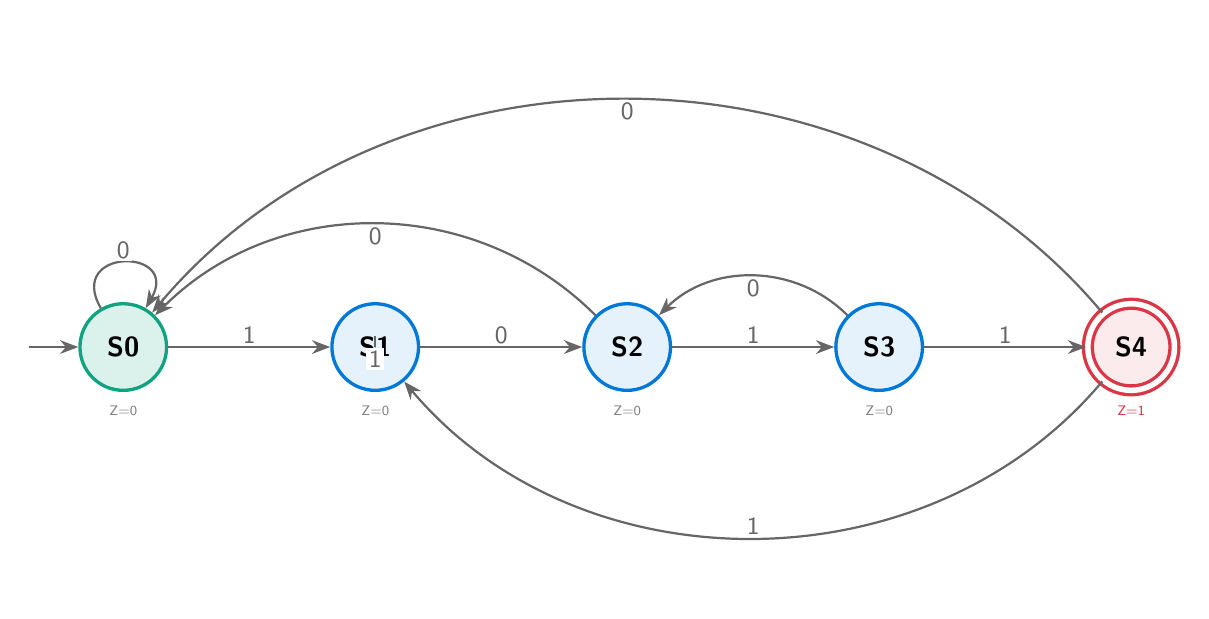
\begin{tikzpicture}[node distance=3.2cm]
  % States
  \node[fsminitial]          (S0) {S0};
  \node[fsmstate, right of=S0] (S1) {S1};
  \node[fsmstate, right of=S1] (S2) {S2};
  \node[fsmstate, right of=S2] (S3) {S3};
  \node[fsmfinal, right of=S3] (S4) {S4};

  % Moore outputs
  \node[below=0.05cm of S0, font=\sffamily\tiny\color{gray}]{Z=0};
  \node[below=0.05cm of S1, font=\sffamily\tiny\color{gray}]{Z=0};
  \node[below=0.05cm of S2, font=\sffamily\tiny\color{gray}]{Z=0};
  \node[below=0.05cm of S3, font=\sffamily\tiny\color{gray}]{Z=0};
  \node[below=0.05cm of S4, font=\sffamily\tiny\color{accentred}]{Z=1};

  % Reset arrow
  \draw[fsmarrow] (-1.2,0) -- (S0);

  % Forward transitions (1,0,1,1)
  \draw[fsmarrow] (S0) to node[fsmlabel, above]{\small 1} (S1);
  \draw[fsmarrow] (S1) to node[fsmlabel, above]{\small 0} (S2);
  \draw[fsmarrow] (S2) to node[fsmlabel, above]{\small 1} (S3);
  \draw[fsmarrow] (S3) to node[fsmlabel, above]{\small 1} (S4);

  % Self-loops / back-transitions
  \draw[fsmarrow] (S0) to[out=120, in=60, looseness=4]
        node[fsmlabel, above]{\small 0} (S0);
  \draw[fsmarrow, bend right=40] (S1) to
        node[fsmlabel, below]{\small 1} (S1);
  \draw[fsmarrow, bend right=45] (S2) to
        node[fsmlabel, below]{\small 0} (S0);
  \draw[fsmarrow, bend right=45] (S3) to
        node[fsmlabel, below]{\small 0} (S2);
  \draw[fsmarrow, bend left=50] (S4) to
        node[fsmlabel, above]{\small 1} (S1);
  \draw[fsmarrow, bend right=50] (S4) to
        node[fsmlabel, below]{\small 0} (S0);
\end{tikzpicture}
\end{center}

\subsection{State Meaning Table}

\begin{center}
\begin{tabular}{cll}
  \toprule
  \textbf{State} & \textbf{Meaning} & \textbf{Bits seen so far} \\
  \midrule
  S0 & Reset / no prefix matched & --- \\
  S1 & Received \texttt{1}       & \texttt{1} \\
  S2 & Received \texttt{10}      & \texttt{10} \\
  S3 & Received \texttt{101}     & \texttt{101} \\
  S4 & Received \texttt{1011}    & \texttt{1011} \textbf{(MATCH!)} \\
  \bottomrule
\end{tabular}
\end{center}

\subsection{VHDL Implementation}

\begin{tcolorbox}[vhdlbox, title={Level 2 --- seq\_detector\_1011.vhd}]
\begin{lstlisting}[style=vhdlstyle]
library ieee;
use ieee.std_logic_1164.all;

entity seq_detector_1011 is
    port (
        clk   : in  std_logic;
        reset : in  std_logic;
        X     : in  std_logic;
        Z     : out std_logic
    );
end seq_detector_1011;

architecture myfsm of seq_detector_1011 is
    -- state encoding
    type state_type is (S0, S1, S2, S3, S4);

    -- signals
    signal state, nextState : state_type;

begin

    -- -----------------------------------------
    -- Process 1 : State Register
    -- -----------------------------------------
    process (reset, clk)
    begin
        if reset = '1' then
            state <= S0;
        elsif rising_edge(clk) then
            state <= nextState;
        end if;
    end process;

    -- -----------------------------------------
    -- Process 2 : Next-State Logic
    -- -----------------------------------------
    process (state, X)
    begin
        -- defaults
        nextState <= S0;
        Z         <= '0';

        case state is

            -- S0 : no bits matched yet
            when S0 =>
                Z <= '0';
                if X = '1' then
                    nextState <= S1;   -- got '1'
                else
                    nextState <= S0;   -- got '0', stay
                end if;

            -- S1 : matched '1'
            when S1 =>
                Z <= '0';
                if X = '0' then
                    nextState <= S2;   -- got '10'
                else
                    nextState <= S1;   -- got '11', restart at '1'
                end if;

            -- S2 : matched '10'
            when S2 =>
                Z <= '0';
                if X = '1' then
                    nextState <= S3;   -- got '101'
                else
                    nextState <= S0;   -- got '100', reset
                end if;

            -- S3 : matched '101'
            when S3 =>
                Z <= '0';
                if X = '1' then
                    nextState <= S4;   -- got '1011'!
                else
                    nextState <= S2;   -- got '1010', overlap at '10'
                end if;

            -- S4 : full match '1011' found
            when S4 =>
                Z <= '1';             -- assert output for 1 cycle
                if X = '1' then
                    nextState <= S1;   -- '1' could start new match
                else
                    nextState <= S0;
                end if;

            when others =>
                nextState <= S0;
                Z         <= '0';

        end case;
    end process;

end myfsm;
\end{lstlisting}
\end{tcolorbox}

\newpage

% ==============================================
%  SECTION 4  —  LEVEL 3
% ==============================================
\section{Level 3 --- Mealy Machine}

\levelbadge{\faUnlock\ Level 3 $\cdot$ Intermediate --- Mealy Output on Transitions}{accentblue!70!black}

\subsection{Moore vs Mealy --- Visual Comparison}

\begin{center}
\begin{tikzpicture}[node distance=4cm]
  %--- Moore (left side) ---
  \node[fsminitial] (MA) {S0};
  \node[fsmstate, right of=MA] (MB) {S1};
  \node[below=0.05cm of MA, font=\sffamily\tiny\color{accentgreen}]{Z=0};
  \node[below=0.05cm of MB, font=\sffamily\tiny\color{accentred}]{Z=1};
  \draw[fsmarrow] (-1.2,0) -- (MA);
  \draw[fsmarrow, bend left=30] (MA) to node[fsmlabel, above]{\small X=1} (MB);
  \draw[fsmarrow, bend left=30] (MB) to node[fsmlabel, below]{\small X=0} (MA);
  \node[above=1.2cm of MA, font=\sffamily\bfseries\color{accentblue}]
       at ($(MA)!0.5!(MB)$) {Moore: output inside state};

  %--- Mealy (right side) ---
  \node[fsminitial, right=7cm of MA] (CA) {S0};
  \node[fsmstate, right of=CA] (CB) {S1};
  \draw[fsmarrow] ($(CA)+(-1.2,0)$) -- (CA);
  \draw[fsmarrow, bend left=30] (CA) to
        node[fsmlabel, above]{\small X=1 / Z=1} (CB);
  \draw[fsmarrow, bend left=30] (CB) to
        node[fsmlabel, below]{\small X=0 / Z=0} (CA);
  \node[above=1.2cm of CA, font=\sffamily\bfseries\color{accentblue!70!black}]
       at ($(CA)!0.5!(CB)$) {Mealy: output on arrow};
\end{tikzpicture}
\end{center}

\subsection{Problem --- Same Sequence Detector, Mealy Style}

Detect \textbf{``1011''} using a \textbf{Mealy} machine.
Output \texttt{Z = 1} is asserted \textit{on the transition} when the
last bit is received, not in a dedicated output state.
This saves one state compared to the Moore version.

\subsection{VHDL Implementation}

\begin{tcolorbox}[vhdlbox, title={Level 3 --- mealy\_1011.vhd}]
\begin{lstlisting}[style=vhdlstyle]
library ieee;
use ieee.std_logic_1164.all;

entity mealy_1011 is
    port (
        clk   : in  std_logic;
        reset : in  std_logic;
        X     : in  std_logic;
        Z     : out std_logic
    );
end mealy_1011;

architecture myfsm of mealy_1011 is
    -- state encoding (one fewer state than Moore!)
    type state_type is (S0, S1, S2, S3);

    -- signals
    signal state, nextState : state_type;

begin

    -- -----------------------------------------
    -- Process 1 : State Register
    -- -----------------------------------------
    process (reset, clk)
    begin
        if reset = '1' then
            state <= S0;
        elsif rising_edge(clk) then
            state <= nextState;
        end if;
    end process;

    -- -----------------------------------------
    -- Process 2 : Next-State + Output (Mealy)
    -- Output Z is assigned on the TRANSITION
    -- -----------------------------------------
    process (state, X)
    begin
        -- defaults
        nextState <= S0;
        Z         <= '0';

        case state is

            -- S0 : no prefix
            when S0 =>
                if X = '1' then
                    nextState <= S1;
                    Z         <= '0';
                else
                    nextState <= S0;
                    Z         <= '0';
                end if;

            -- S1 : matched '1'
            when S1 =>
                if X = '0' then
                    nextState <= S2;
                    Z         <= '0';
                else
                    nextState <= S1;   -- '11' -> keep '1'
                    Z         <= '0';
                end if;

            -- S2 : matched '10'
            when S2 =>
                if X = '1' then
                    nextState <= S3;
                    Z         <= '0';
                else
                    nextState <= S0;
                    Z         <= '0';
                end if;

            -- S3 : matched '101'
            when S3 =>
                if X = '1' then
                    nextState <= S1;   -- overlap: last '1' starts new match
                    Z         <= '1';  -- OUTPUT HERE on the transition!
                else
                    nextState <= S2;   -- '1010' -> overlap at '10'
                    Z         <= '0';
                end if;

            when others =>
                nextState <= S0;
                Z         <= '0';

        end case;
    end process;

end myfsm;
\end{lstlisting}
\end{tcolorbox}

\begin{tcolorbox}[notebox, title={Mealy Key Point}]
  In Mealy, \texttt{Z} is assigned \textbf{inside the transition condition}
  (\texttt{if X = '1' then ... Z <= '1'}).
  It can change \textit{between} clock edges whenever \texttt{X} changes.
  This is why Mealy needs one fewer state but can produce glitches on output.
\end{tcolorbox}

\newpage

% ==============================================
%  SECTION 5  —  LEVEL 4
% ==============================================
\section{Level 4 --- 3-Process FSM \& Multiple Outputs}

\levelbadge{\faUnlock\ Level 4 $\cdot$ Intermediate-Advanced --- 3-Process Style}{accentblue!50!black}

\subsection{Why a Third Process?}

The 2-process style mixes next-state logic and output logic in one process.
The \textbf{3-process} style separates them for clarity and avoids
accidental latch inference in large FSMs.

\begin{center}
\begin{tabular}{clp{7cm}}
  \toprule
  \textbf{Process} & \textbf{Sensitive to} & \textbf{Responsibility} \\
  \midrule
  1 & \texttt{reset, clk}  & State register (flip-flops only) \\
  2 & \texttt{state, inputs} & Next-state logic only \\
  3 & \texttt{state} (Moore) or \texttt{state, inputs} (Mealy)
    & Output logic only \\
  \bottomrule
\end{tabular}
\end{center}

\subsection{Problem --- Traffic Light Controller}

A simple 3-state traffic light: \textbf{Green} $\to$ \textbf{Yellow}
$\to$ \textbf{Red} $\to$ \textbf{Green} $\ldots$
Input \texttt{timer} goes high when the current phase times out.
Outputs: \texttt{green}, \texttt{yellow}, \texttt{red}.

\begin{tcolorbox}[vhdlbox, title={Level 4 --- traffic\_light.vhd}]
\begin{lstlisting}[style=vhdlstyle]
library ieee;
use ieee.std_logic_1164.all;

entity traffic_light is
    port (
        clk    : in  std_logic;
        reset  : in  std_logic;
        timer  : in  std_logic;   -- '1' when phase timer expires
        green  : out std_logic;
        yellow : out std_logic;
        red    : out std_logic
    );
end traffic_light;

architecture myfsm of traffic_light is
    -- state encoding
    type state_type is (GREEN, YELLOW, RED);

    -- signals
    signal state, nextState : state_type;

begin

    -- -----------------------------------------
    -- Process 1 : State Register
    -- -----------------------------------------
    process (reset, clk)
    begin
        if reset = '1' then
            state <= GREEN;
        elsif rising_edge(clk) then
            state <= nextState;
        end if;
    end process;

    -- -----------------------------------------
    -- Process 2 : Next-State Logic ONLY
    -- -----------------------------------------
    process (state, timer)
    begin
        nextState <= state;   -- default: hold state

        case state is

            when GREEN =>
                if timer = '1' then
                    nextState <= YELLOW;
                end if;

            when YELLOW =>
                if timer = '1' then
                    nextState <= RED;
                end if;

            when RED =>
                if timer = '1' then
                    nextState <= GREEN;
                end if;

            when others =>
                nextState <= GREEN;

        end case;
    end process;

    -- -----------------------------------------
    -- Process 3 : Output Logic ONLY (Moore)
    -- Sensitive only to state (pure Moore)
    -- -----------------------------------------
    process (state)
    begin
        -- default all outputs off
        green  <= '0';
        yellow <= '0';
        red    <= '0';

        case state is
            when GREEN  => green  <= '1';
            when YELLOW => yellow <= '1';
            when RED    => red    <= '1';
            when others => null;
        end case;
    end process;

end myfsm;
\end{lstlisting}
\end{tcolorbox}

\begin{tcolorbox}[notebox, title={3-Process Advantages}]
  \begin{itemize}
    \item Output process is \textbf{pure combinational} and easy to read.
    \item Changing output logic never accidentally touches next-state logic.
    \item Synthesis tools can optimize each process independently.
    \item Easier to convert between Moore and Mealy (just change Process 3).
  \end{itemize}
\end{tcolorbox}

\newpage

% ==============================================
%  SECTION 6  —  LEVEL 5
% ==============================================
\section{Level 5 --- State Encoding Strategies}

\levelbadge{\faUnlock\ Level 5 $\cdot$ Advanced --- Binary, Gray Code, One-Hot}{accentred!70!black}

\subsection{Three Encoding Methods}

VHDL lets you declare states symbolically and let the tool choose encoding,
or you can \textbf{force} a specific encoding using constants.

\begin{center}
\begin{tabular}{lccc}
  \toprule
  \textbf{Method} & \textbf{Bits needed} & \textbf{Flip-flops} & \textbf{Best for} \\
  \midrule
  Binary   & $\lceil \log_2 N \rceil$ & Fewest    & Low resource designs \\
  Gray     & $\lceil \log_2 N \rceil$ & Fewest    & Low EMI / glitch sensitive \\
  One-Hot  & $N$                      & Most      & Fast FPGAs (LUT efficiency) \\
  \bottomrule
\end{tabular}
\end{center}

\subsection{Forcing Encoding in VHDL}

\begin{tcolorbox}[vhdlbox, title={Level 5 --- state\_encoding.vhd}]
\begin{lstlisting}[style=vhdlstyle]
library ieee;
use ieee.std_logic_1164.all;

-- ---------------------------------------------
-- METHOD A : Binary Encoding (manual)
-- 3 states need 2 bits: S0=00, S1=01, S2=10
-- ---------------------------------------------
architecture binary_enc of fsm_enc is

    constant S0 : std_logic_vector(1 downto 0) := "00";
    constant S1 : std_logic_vector(1 downto 0) := "01";
    constant S2 : std_logic_vector(1 downto 0) := "10";

    signal state, nextState : std_logic_vector(1 downto 0);

begin
    -- processes same as before, just use std_logic_vector
    process (reset, clk)
    begin
        if reset = '1' then
            state <= S0;
        elsif rising_edge(clk) then
            state <= nextState;
        end if;
    end process;

    process (state, X)
    begin
        nextState <= S0;
        Z         <= '0';

        case state is
            when S0 =>
                if X = '1' then nextState <= S1; end if;
            when S1 =>
                if X = '1' then nextState <= S2;
                else            nextState <= S0; end if;
            when S2 =>
                Z <= '1';
                nextState <= S0;
            when others =>
                nextState <= S0;
        end case;
    end process;

end binary_enc;


-- ---------------------------------------------
-- METHOD B : One-Hot Encoding
-- 3 states need 3 bits: S0=001, S1=010, S2=100
-- ---------------------------------------------
architecture onehot_enc of fsm_enc is

    constant S0 : std_logic_vector(2 downto 0) := "001";
    constant S1 : std_logic_vector(2 downto 0) := "010";
    constant S2 : std_logic_vector(2 downto 0) := "100";

    signal state, nextState : std_logic_vector(2 downto 0);

begin
    process (reset, clk)
    begin
        if reset = '1' then
            state <= S0;       -- only bit 0 set
        elsif rising_edge(clk) then
            state <= nextState;
        end if;
    end process;

    process (state, X)
    begin
        nextState <= S0;
        Z         <= '0';

        case state is
            when S0 =>
                if X = '1' then nextState <= S1; end if;
            when S1 =>
                if X = '1' then nextState <= S2;
                else            nextState <= S0; end if;
            when S2 =>
                Z <= '1';
                nextState <= S0;
            when others =>
                nextState <= S0;  -- fault recovery
        end case;
    end process;

end onehot_enc;


-- ---------------------------------------------
-- METHOD C : Let Quartus decide (RECOMMENDED)
-- Add synthesis attribute in your QSF file:
--   set_global_assignment -name STATE_MACHINE_PROCESSING ONE-HOT
-- Or use the Quartus GUI: Assignments > Settings >
--   Compiler Settings > Advanced Settings (Synthesis)
-- ---------------------------------------------
architecture auto_enc of fsm_enc is

    -- Just use enumerated type; Quartus picks best encoding
    type state_type is (S0, S1, S2);
    signal state, nextState : state_type;

begin
    -- ... same 2-process template ...
end auto_enc;
\end{lstlisting}
\end{tcolorbox}

\newpage

% ==============================================
%  SECTION 7  —  LEVEL 6
% ==============================================
\section{Level 6 --- FSM with Datapath (FSMD)}

\levelbadge{\faStar\ Level 6 $\cdot$ Advanced --- FSM + Counter/Register Datapath}{accentred}

\subsection{What is an FSMD?}

In real designs, an FSM alone is not enough. You combine an FSM
(\textbf{controller}) with a \textbf{datapath} (counters, registers,
adders) to build complex digital systems.

\begin{center}
\begin{tikzpicture}
  \node[draw=accentblue, fill=accentblue!10, rounded corners,
        minimum width=3.5cm, minimum height=1.8cm, align=center,
        font=\sffamily\bfseries] (ctrl)
        {FSM\\Controller};

  \node[draw=accentred, fill=accentred!10, rounded corners,
        minimum width=3.5cm, minimum height=1.8cm, align=center,
        font=\sffamily\bfseries, right=5cm of ctrl] (dp)
        {Datapath\\(counter / register)};

  \draw[fsmarrow, bend left=25] (ctrl) to
        node[fsmlabel, above]{\small control signals}  (dp);
  \draw[fsmarrow, bend left=25] (dp)   to
        node[fsmlabel, below]{\small status signals}   (ctrl);

  \draw[fsmarrow] ($(ctrl)+(-1.8,0.3)$) -- node[fsmlabel,above]{\small inputs}  ($(ctrl)+(-0.1,0.3)$);
  \draw[fsmarrow] ($(ctrl)+(-0.1,-0.3)$) -- node[fsmlabel,below]{\small outputs} ($(ctrl)+(-1.8,-0.3)$);
\end{tikzpicture}
\end{center}

\subsection{Problem --- Pulse-Width Counter}

Count how many clock cycles input \texttt{X} stays high.
When \texttt{X} goes low, output the 4-bit count \texttt{CNT} and
assert \texttt{done = 1} for one cycle.

\begin{tcolorbox}[vhdlbox, title={Level 6 --- pulse\_counter\_fsmd.vhd}]
\begin{lstlisting}[style=vhdlstyle]
library ieee;
use ieee.std_logic_1164.all;
use ieee.numeric_std.all;        -- needed for unsigned counter

entity pulse_counter_fsmd is
    port (
        clk   : in  std_logic;
        reset : in  std_logic;
        X     : in  std_logic;
        CNT   : out std_logic_vector(3 downto 0);
        done  : out std_logic
    );
end pulse_counter_fsmd;

architecture myfsm of pulse_counter_fsmd is

    -- -- FSM (controller) ----------------------
    type state_type is (IDLE, COUNTING, REPORT);
    signal state, nextState : state_type;

    -- -- Datapath signals ----------------------
    signal count     : unsigned(3 downto 0);
    signal count_en  : std_logic;   -- control: enable counter
    signal count_clr : std_logic;   -- control: clear counter

begin

    -- -----------------------------------------
    -- Datapath : 4-bit counter
    -- -----------------------------------------
    process (reset, clk)
    begin
        if reset = '1' then
            count <= (others => '0');
        elsif rising_edge(clk) then
            if count_clr = '1' then
                count <= (others => '0');
            elsif count_en = '1' then
                count <= count + 1;
            end if;
        end if;
    end process;

    -- -----------------------------------------
    -- Process 1 : State Register
    -- -----------------------------------------
    process (reset, clk)
    begin
        if reset = '1' then
            state <= IDLE;
        elsif rising_edge(clk) then
            state <= nextState;
        end if;
    end process;

    -- -----------------------------------------
    -- Process 2 : Next-State Logic
    -- -----------------------------------------
    process (state, X)
    begin
        nextState <= state;

        case state is
            when IDLE =>
                if X = '1' then
                    nextState <= COUNTING;
                end if;

            when COUNTING =>
                if X = '0' then
                    nextState <= REPORT;
                end if;

            when REPORT =>
                nextState <= IDLE;   -- stay 1 cycle then go idle

            when others =>
                nextState <= IDLE;
        end case;
    end process;

    -- -----------------------------------------
    -- Process 3 : Output + Control Signals
    -- -----------------------------------------
    process (state, count)
    begin
        -- defaults
        count_en  <= '0';
        count_clr <= '0';
        done      <= '0';
        CNT       <= (others => '0');

        case state is
            when IDLE =>
                count_clr <= '1';    -- keep counter cleared

            when COUNTING =>
                count_en  <= '1';    -- increment every cycle X is high

            when REPORT =>
                done <= '1';
                CNT  <= std_logic_vector(count);

            when others =>
                null;
        end case;
    end process;

end myfsm;
\end{lstlisting}
\end{tcolorbox}

\newpage

% ==============================================
%  SECTION 8  —  COMMON MISTAKES
% ==============================================
\section{Common Mistakes \& How to Fix Them}

\begin{tcolorbox}[notebox, title={These bugs were found in a real student file!}]
  The following table documents the \textbf{exact errors} from a typical
  first attempt. Study each one carefully.
\end{tcolorbox}

\subsection{Bug Reference Table}

\begin{center}
\renewcommand{\arraystretch}{1.6}
\begin{tabular}{>{\ttfamily\small}p{4.5cm}
                >{\ttfamily\small\color{accentred}}p{4cm}
                >{\ttfamily\small\color{accentgreen}}p{4cm}}
  \toprule
  \normalfont\textbf{Location} &
  \normalfont\textbf{\faTimesCircle\ Wrong} &
  \normalfont\textbf{\faCheckCircle\ Correct} \\
  \midrule
  Port direction of reset, clk, X &
  reset : out &
  reset : in \\

  Port direction of reset, clk, X &
  X, clk : out &
  X, clk : in \\

  Signal declaration &
  signal state, nextState, stateType ; &
  signal state, nextState : state\_type; \\

  State register if-condition &
  if reset = '1' \newline (missing then) &
  if reset = '1' then \\

  Clock edge function &
  riding\_edge(clk) &
  rising\_edge(clk) \\

  End of if statement &
  end; &
  end if; \\

  Duplicate case branch &
  when S0 => ... \newline when S0 => ... &
  Each state appears \newline exactly ONCE \\

  Missing output state &
  when S2 missing ... &
  Every declared state \newline must have a when \\

  Missing catch-all &
  (no when others) &
  when others => \newline nextState <= S0; \\

  Architecture end &
  end myfsm &
  end myfsm; \\

  \bottomrule
\end{tabular}
\end{center}

\subsection{The Corrected Version of Your fsm.vhd}

\begin{tcolorbox}[vhdlbox, title={fsm.vhd --- Corrected}]
\begin{lstlisting}[style=vhdlstyle]
library ieee;
use ieee.std_logic_1164.all;

entity fsm is
    port (
        clk   : in  std_logic;   -- FIX: was "out"
        reset : in  std_logic;   -- FIX: was "out"
        X     : in  std_logic;   -- FIX: was "out"
        Z     : out std_logic
    );
end fsm;

architecture myfsm of fsm is
    -- state encoding
    type state_type is (S0, S1, S2, S3, S4, S5, S6);

    -- FIX: missing ": state_type" and removed stateType
    signal state, nextState : state_type;

begin

    -- -----------------------------------------
    -- Process 1 : State Register
    -- -----------------------------------------
    process (reset, clk)
    begin
        if reset = '1' then       -- FIX: added "then"
            state <= S0;
        elsif rising_edge(clk) then   -- FIX: "riding" -> "rising"
            state <= nextState;
        end if;                   -- FIX: "end;" -> "end if;"
    end process;

    -- -----------------------------------------
    -- Process 2 : Next-State + Output Logic
    -- -----------------------------------------
    process (state, X)
    begin
        -- defaults prevent latches
        nextState <= S0;
        Z         <= '0';

        case state is

            -- S0
            when S0 =>
                if X = '0' then
                    nextState <= S1;
                    Z         <= '1';
                else
                    nextState <= S0;
                    Z         <= '0';
                end if;

            -- S1
            when S1 =>
                if X = '0' then
                    nextState <= S3;
                    Z         <= '1';
                else
                    nextState <= S4;
                    Z         <= '0';
                end if;

            -- S2
            when S2 =>
                if X = '0' then
                    nextState <= S4;
                    Z         <= '0';
                else
                    nextState <= S4;
                    Z         <= '1';
                end if;

            -- FIX: S3, S4, S5, S6 all need their own when clause
            when S3 =>
                nextState <= S0;
                Z         <= '0';

            when S4 =>
                nextState <= S0;
                Z         <= '0';

            when S5 =>
                nextState <= S0;
                Z         <= '0';

            when S6 =>
                nextState <= S0;
                Z         <= '0';

            -- FIX: always include when others
            when others =>
                nextState <= S0;
                Z         <= '0';

        end case;
    end process;

end myfsm;   -- FIX: added semicolon
\end{lstlisting}
\end{tcolorbox}

\newpage

% ==============================================
%  SECTION 9  —  QUICK REFERENCE
% ==============================================
\section{Quick Reference --- The Master Template}

\begin{tcolorbox}[vhdlbox, title={Master 2-Process FSM Template (Copy \& Adapt)}]
\begin{lstlisting}[style=vhdlstyle]
library ieee;
use ieee.std_logic_1164.all;

entity YOUR_FSM_NAME is
    port (
        clk   : in  std_logic;
        reset : in  std_logic;
        -- add your inputs here  (always "in")
        -- add your outputs here (always "out")
    );
end YOUR_FSM_NAME;

architecture myfsm of YOUR_FSM_NAME is
    type state_type is (S0, S1, S2 /*, add more states */);
    signal state, nextState : state_type;

begin

    -- -----------------------------------------
    -- Process 1 : State Register  [NEVER changes]
    -- -----------------------------------------
    process (reset, clk)
    begin
        if reset = '1' then
            state <= S0;
        elsif rising_edge(clk) then
            state <= nextState;
        end if;
    end process;

    -- -----------------------------------------
    -- Process 2 : Next-State + Output  [All logic here]
    -- -----------------------------------------
    process (state /*, add all inputs to sensitivity list */)
    begin
        -- ALWAYS write defaults first
        nextState <= S0;
        -- YOUR_OUTPUT <= '0';

        case state is

            when S0 =>
                -- YOUR_OUTPUT <= ...;
                if (/* condition */) then
                    nextState <= S1;
                else
                    nextState <= S0;
                end if;

            when S1 =>
                -- add more states ...
                nextState <= S0;

            -- ALWAYS include this
            when others =>
                nextState <= S0;

        end case;
    end process;

end myfsm;
\end{lstlisting}
\end{tcolorbox}

\subsection{FSM Design Checklist}

\begin{tcolorbox}[successbox, title={\faCheckSquare\ Before You Synthesize --- Run This Checklist}]
  \begin{enumerate}[leftmargin=1.5cm]
    \item[\faCheck] All ports: \texttt{clk}, \texttt{reset}, inputs are \texttt{in};
                   outputs are \texttt{out}.
    \item[\faCheck] Signal declaration: \texttt{signal state, nextState : state\_type;}
                   (type specified!).
    \item[\faCheck] State register uses \texttt{rising\_edge(clk)} (not \texttt{riding\_edge}).
    \item[\faCheck] State register if-clause ends with \texttt{end if;} (not \texttt{end;}).
    \item[\faCheck] Every state in \texttt{state\_type} has exactly \textbf{one}
                   \texttt{when} clause.
    \item[\faCheck] \texttt{when others} is the last clause in every \texttt{case}.
    \item[\faCheck] Default assignments written at the \textbf{top} of Process 2.
    \item[\faCheck] All inputs added to the sensitivity list of Process 2.
    \item[\faCheck] Architecture ends with \texttt{end myfsm;} (semicolon!).
    \item[\faCheck] No duplicate \texttt{when} labels in any \texttt{case} block.
    \item[\faCheck] Outputs never driven from Process 1 (state register).
  \end{enumerate}
\end{tcolorbox}

\subsection{Level Summary Table}

\begin{center}
\renewcommand{\arraystretch}{1.5}
\begin{tabular}{clccp{4.5cm}}
  \toprule
  \textbf{Level} & \textbf{Topic} & \textbf{States} & \textbf{Processes} & \textbf{New Skill} \\
  \midrule
  1 & Toggle (Moore)          & 2   & 2 & Basic template, port directions \\
  2 & Sequence Detector Moore & 5   & 2 & Multi-state, overlapping detection \\
  3 & Sequence Detector Mealy & 4   & 2 & Output on transitions, fewer states \\
  4 & Traffic Light (3-proc)  & 3   & 3 & Separated output process, multi-output \\
  5 & State Encoding          & Any & 2 & Binary, Gray, One-Hot, auto \\
  6 & FSMD Pulse Counter      & 3   & 3+ & FSM + datapath, control signals \\
  \bottomrule
\end{tabular}
\end{center}

\subsection{The Golden Rules (Never Break These)}

\begin{tcolorbox}[errorbox, title={\faExclamationTriangle\ The 5 Rules You Must Never Break}]
  \begin{enumerate}[leftmargin=1.5cm]
    \item \textbf{Never} drive the same signal from two different processes.
    \item \textbf{Never} put \texttt{rising\_edge} in a combinational process
          (Process 2 or 3).
    \item \textbf{Always} write default assignments before \texttt{case} in
          any combinational process --- avoids inferred latches.
    \item \textbf{Always} include \texttt{when others} --- an FPGA can power up
          in an unknown state.
    \item \textbf{Never} read an output port inside the architecture --- declare
          an internal signal, drive the output from it.
  \end{enumerate}
\end{tcolorbox}

\vfill
\begin{center}
  \color{gray}\sffamily\small
  \noindent\rule{0.6\linewidth}{0.4pt}\\[4pt]
  FSM in VHDL --- Complete Guide $\cdot$ DSD Lab $\cdot$
  Built with \LaTeX\ + TikZ
\end{center}

\end{document}
